\documentclass{article}
% set margins
\usepackage[left=1.5in, right=1in, top=1in, bottom=1in]{geometry}
% add spacing
\usepackage{setspace}
% use biblatex
\usepackage[style=numeric]{biblatex}
% add the bibliography
\addbibresource{bibliography.bib}
% remove dots in TOC
\usepackage[titles]{tocloft}
\renewcommand{\cftdot}{}

\usepackage{amssymb}
\usepackage{amsmath}

% unbold things
\usepackage{titlesec}
\titleformat*{\section}\MakeUppercase{\normalfont}
\titleformat*{\subsection}{\em {\normalfont} }
\titleformat*{\subsubsection}{\normalfont}

\usepackage{graphicx}
\graphicspath{ {images/} }

\title{Exploring Semantic Hierarchies to Improve Resolution Theorem Proving on Ontologies}
\author{Stanley C. Small}
\date{March 2019}

\begin{document}
	\begin{titlepage}
		\makeatletter
			\begin{center}
       				\MakeUppercase{\@title} \par
      				\smallskip 
     				\vspace{.15in} by \par
     				\smallskip
      				\vspace{.15in} \@author \par
      				\vspace{1in}
     				A Thesis Submitted in Partial Fulfillment  \par
      				of the Requirements for a Degree with Honors \par
      				(Computer Science) \par
      				\vspace{.75in}
      				The Honors College \par
      				University of Maine \par
      				\@date \par
     				\vfill
   			\end{center}
		\makeatother
		\begin{flushleft}
			Advisory Committee: \\
			\hspace{.3in} Dr. Torsten Hahmann, Professor of Things, Advisor \\
			\hspace{.3in} Dr. Mark Brewer, Professor of Things \\
			\hspace{.3in} Dr. Max Egenhofer, Professor of Things \\
			\hspace{.3in} Dr. Sepideh Ghanavati, Professor of Things \\
			\hspace{.3in} Dr. Roy Turner, Professor of Things
		\end{flushleft}
	\end{titlepage}
	
	\pagenumbering{gobble}
	\newpage
	\setstretch{2}
	\section*{Abstract}
A resolution-theorem-prover (RTP) evaluates the validity (truthfulness) of conjectures against a set of axioms classified as a knowledgebase. When given a conjecture, an RTP attempts to resolve the negated conjecture with axioms from the knowledge-base until the prover finds a contradiction. If the RTP finds a contradiction between the axioms and a negated conjecture, it proves the conjecture. 

The order in which the axioms within the knowledge-base are evaluated significantly impacts the runtime of the program, as the search-space increases exponentially with the number of axioms. 

Ontologies, knowledge bases with semantic (and predominantly hierarchical) structures, describe objects and their relationships to other objects. For example, a 'Car' class might exist in a sample ontology with 'Vehicle' as a parent class and 'Bus' as a sibling class. Currently, any hierarchical structures within an ontology are not taken into account when evaluating the relevance of each axiom. At present, each predicate is automatically assigned a weight based on a heuristic measure (such as the number of terms or the frequency of predicates relevant to the conjecture) and axioms with higher weights are evaluated first. My research aims to intelligently select relevant axioms within a knowledge-base given a structured relationship between predicates. I will use the semantic hierarchy over predicates to assign weights to each predicate passed to a weighting function. The research aims to design heuristics based upon the semantics of the predicates, rather than solely the syntax of the statements. 

I plan to develop weighting functions based upon various parameters relevant to the ontological structure of predicates contained in the ontology, such as the size and depth of a hierarchy based upon the structure of the ontology. 

I will implement methods to calculate weights for each predicate and thus each axiom in attempts to select relevant axioms when proving a theorem. Then, I will conduct an experimental study to determine if my methods show any improvements over current reasoning methods.
	
	\pagenumbering{roman} 
	\setcounter{page}{3}
        \newpage
        \section*{Acknowledgements}
Many thanks are given to Dr. Hahmann. This work could not be completed without his continued support and encouragement. Despite his tremendously busy schedule, he always made time to meet and answer questions. 

Robert Powell also proved instrumental to the process. His utility which converts Common Logic Interchange Format (CLIF) into web ontology language (OWL). His work streamlined the testing process and allowed me to find necessary results. 

The thesis committee was also instrumental in producing this undergraduate thesis.

	\newpage
	\listoffigures

	\newpage
	\setstretch{1.5}
	\tableofcontents

	\newpage
	\setstretch{2}
	\pagenumbering{arabic}
	\setcounter{page}{1}
	\section{Introduction}

%Generally, try to expand more and clearly separate the text into modular units: 1) what is theorem proving 2) applications of theorem proving 3) what are ontologies 4) what role does theorem proving play with ontologies 5) what is so special about theorem proving with ontologies.

%Try to use some very simple examples, e.g., a toy ontology, specific domains for ontologies, the kind of relations we can find therein (subclass and subproperty, domain and range restrictions), what the semantic hierarchy looks in the example, an example how the semantic hierarchy may help in a proof (when there are lots of irrelevant axioms).

A theorem is a statement that can be proved from a series of asserted facts, typically referred to as axioms, using the rules of logic. By expressing facts in a formal manner, new statements can be generated mechanically by a computer program without additional user input. Computers excel at tasks which remain simple and repetitive. Formal logic defines rules of inference which allow one to transform established facts into new conclusions based on the syntax of these statements. Such inference rules are relatively easy to implement in a computer program because these rules rely only on the syntax, or the structure, of facts instead of any sense of meaning inherent in a set of facts. This is referred to as automated theorem proving. Automated theorem proving provides a versatile method for reasoning with a set of facts, and has been used to prove and verify proofs of multiple theorems. The four color map theorem is a notable example of a theorem obtained by an automated proof in 1976, and by a general-purpose theorem-proving software in 2005 \cite{gonthier2008formal}. Moreover, advances have been made in work on the Kepler conjecture and in finding optimal solutions for a Rubik's Cube with computer programs using formal reasoning methods. 

ONTOLOGIES AIM TO CAPTURE THE SEMANTICS OF A DOMAIN'S CONCEPTS AND RELATIONS. The general-purpose nature of automated theorem proving makes the method applicable to a variety of problems, but a considerable amount of information is lost when applied on ontologies. ONTOLOGIES ARE SETS OF AXIOMS. An ontology is a set of facts describing entities and the relationships between them. Some relationships between an ontology's terms may be explicitly defined, but many are implicit. EXAMPLE OF RELATIONSHIP. Relationships between entities can often be represented as a tree, and more specifically a hierarchy. Encoded in the hierarchy is a wealth of information detailing the relationships between entities described in an ontology. Currently, knowledge encoded in structural hierarchies constructed from ontologies is not taken into account when determining which axioms might be most helpful when attempting to prove a specific theorem. This work attempts to improve automated theorem proving with ontologies by identifying relevant facts, and ignoring those less likely to yield a proof. DESCRIPTION OF THE CONCRETE OBJECTIVE AND APPROACH OF YOUR WORK


	\newpage
	\section{Background and Related Work}

		\subsection{Ontologies}
		
Ontologies describe entities and relationships between them. The explicit description of a specific environment provides researchers and machines a shared understanding of said environment. The word ontology ("study of being") combines Greek \textit{onto-} ("being") and \textit{-logia} ("logical discourse"). The act of studying knowledge and existence in philosophy has given birth to the study of formal logic and automated reasoning in computer science. Ontologies provide a "common vocabulary" for researchers to speak about a specific domain \cite{noy2001ontology}. Furthermore, ontologies can often be interpreted by machines to aid in automated proofs. While ontologies at a fundamental level exist as a collection of facts, the organization and descriptions which researchers choose to represent a specific domain are important. Perhaps an ontology can best be understood with an example inspired by an example composed by Natalya F. Noy \cite{noy2001ontology}. 

\begin{figure}[h]
\centering
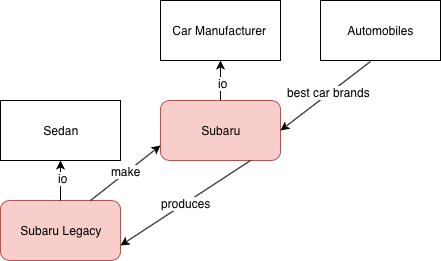
\includegraphics[scale=.5]{sample_ontology}
\caption{This is a simple ontology describing classes (black) and instances (red) in the "automobiles" ontology.}
\label{fig:sample_ontology}
\end{figure}

		\subsection{Theorem Proving}
Formal logic, specifically first-order logic, defines a structure for statements which can be used to form logical and mathematical proofs. Asserted facts, called axioms, are used to derive facts which logically follow. Consider the following set of facts. 
\begin{singlespace}
        \[isSedan(Subaru Legacy)\]
        \[isSedan(X) \rightarrow hasFourSeats(X)\]
 \end{singlespace} 
        
The first statement asserts the Subaru Legacy is a sedan. The second statement asserts all sedans have four seats. These two statements do not directly state the Subaru Legacy has four seats. However, one can derive the statement $hasFourSeatsl(Subaru Legacy)$ by using the inference rule \textit{modus ponens}, defined below. 
\begin{singlespace}
	 \[A\]
        \[A \rightarrow B\]
         \[\therefore B\]
\end{singlespace} 

One can think of $A$ and $B$ as variables representing statements, and any statement can replace them. An inference rule defines a valid rule for statements. By expressing facts in a formal notation, one makes proofs using such statements mechanical and easily parsed by a computer. Expressing statements in formal logic poses multiple challenges. First, each object and relationship must be explicitly defined.

Resolution is one of many methods for automated theorem proving. Historically, resolution has significance and is widely used \cite[51]{ertel2018introduction}.
In order to use resolution as a proof technique, axioms must first be expressed in Conjunctive Normal Form. This can be done by expressing the set of facts as a conjunction of disjunctions. 
\begin{singlespace}
		 \[isSedan(X) \rightarrow hasFourSeats(X)\]
		\[\lnot isSedan(X) \lor hasFourSeats(X)\]
		One can then resolve the statements. 
		\[\frac{isSedan(X) \lor hasFourSeats(X), \lnot isSedan(Subaru Legacy)}{hasFourSeats(Subaru Legacy)}\]
\end{singlespace} 
		

In resolution, the search space increases exponentially with the addition of each new axiom. 
Currently only the syntax of statements is taken into account

	

        Syntax defines the structure of a sentence, whereas semantics describe the meaning of a sentence. 
	

		An ontology defines categories and relationships among objects.
		One can think of an ontology as a "vocabulary" used to desrcibe a domain \cite[308]{russell2016artificial}. Typically, the objects can be arranged in a hierarchy. 
		
	At a simplistic level, semantic hierarchies describing an ontology can be compared to a family tree. Given a pair of two individuals, if one were tasking with determining if two individuals are related, a family tree would prove quite useful. 


	\newpage	
	\section{Approach}
		\subsection{Weighting Functions}
Given an ontology and a conjecture, one can generate weights for classes and properties to reduce the number of clauses generated in a proof. Functions are evaluated by their influence on the number of clauses generated with a proof. 

After a hierarchy has been generated, weights can be assigned to each class and subproperty. The same weighting function is applied to both the classes and sub-properties. 

The weighting functions are currently applied by hand to the ontologies, with the beginnings of an automated program underway. 

		\subsection{Computing Weighting Functions}

	\newpage
	\section{Experiments}

\subsection{Setup}
In efforts to quantitatively evaluate the effectiveness of the proposed weighting functions, a series of experiments were conducted on multiple ontologies. The ontologies selected for testing are part of the COmmon Logic Ontology REpository (COLORE). The objective of COLORE is to serve as a "testbed for ontology evaluation and integration techniques" \cite{gruninger2012specifying}. Code from the project can be found at \url{https://code.google.com/archive/p/colore}. 

My experiments were conducted using Prover9, written by William McCune \cite{mccune2005prover9}. Many tests were conducted using a version of the program which supports a GUI, but a command line version is available for running automated tests. 
Git was used for version control and a repository containing source code can be found at \url{https://github.com/stanleysmall/thesis}.

\begin{figure}[h]
\centering
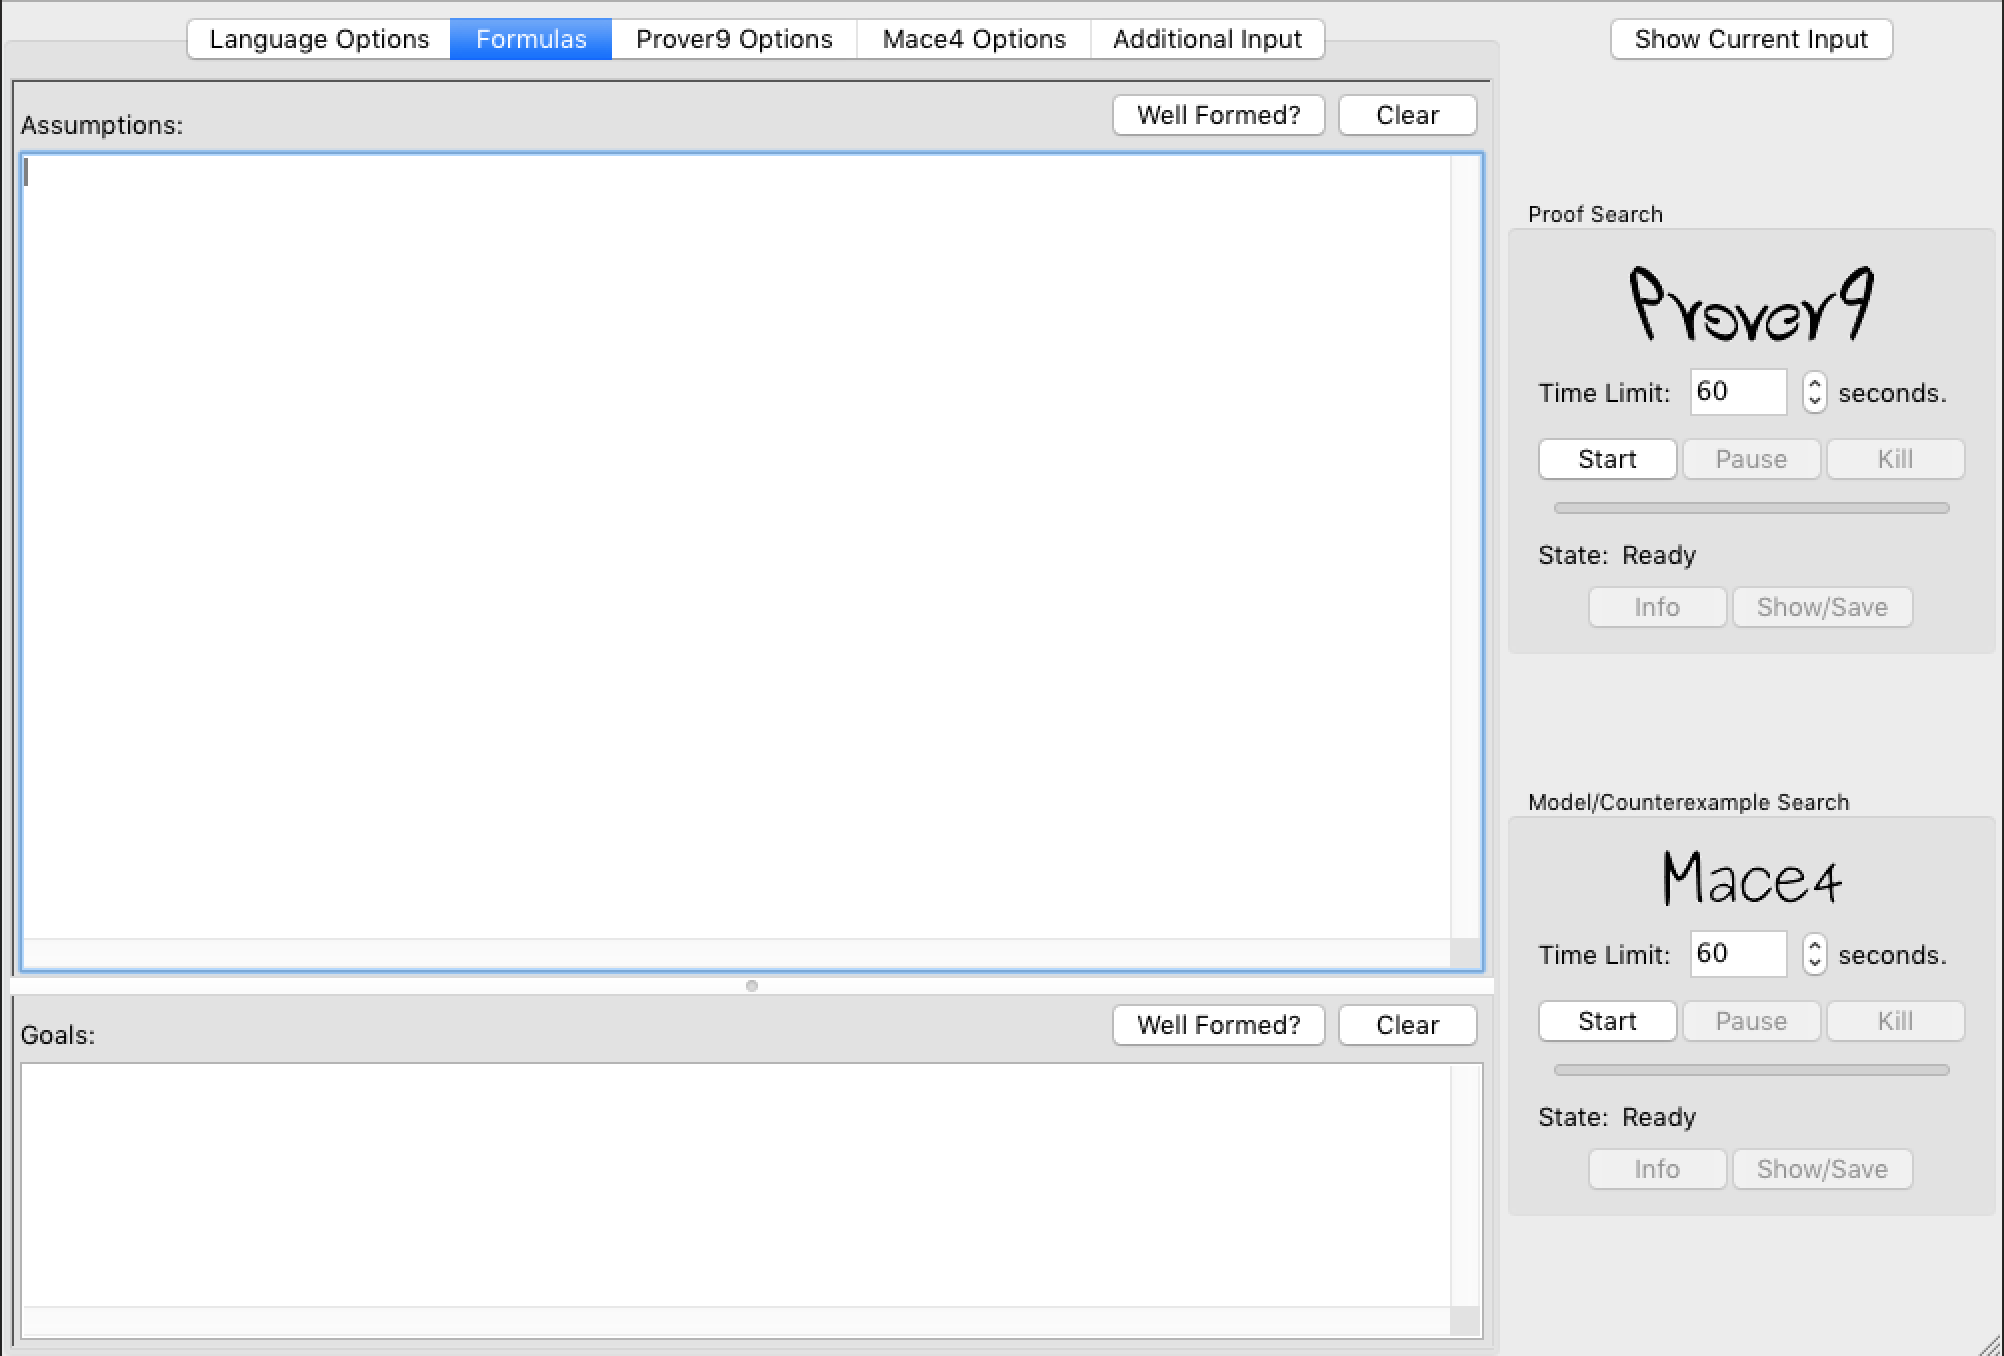
\includegraphics[width=6in]{prover9}
\caption{The graphical user interface for Prover9 on macOS \cite{mccune2005prover9}.}
\label{fig:prover9}
\end{figure}
		



		\subsection{Results}
	\newpage
	\section{Conclusions}

In many cases, the algorithm increases the number of clauses generated for each test, but does not do so to the point where the tests are unusable. For some very specific ontologies, the number of clauses generated decreases. This can be attributed to, in part, by the small number of ontologies available for testing, along with the specific pattern and hierarchy of each ontology. 

Many opportunities for further research include fully automating the search procedure, working with a larger number of ontologies to ensure the weighting functions actually do as they say, developing a new approach towards automatically weighting the predicates. 
	\newpage
	\printbibliography

	\newpage
	\appendix

	\section{Tests}

	\newpage
	\section*{Author's Biography}
Stanley C. Small grew up in Hampden, Maine with his mother Diane and his father Scott. He attended the University of Maine and received a Bachelor of Science degree in Computer Science in May of 2019. 


\end{document}
